\section{Les hypercubes}

Un hypercube est une grille de dimension $d$ ne possédant que deux sommets selon chaque coordonnée. Ainsi, il possède $2^d$ nœuds de degré $d$ et $d2^{d-1}$ arêtes. On construit un hypercube de dimension $d$ récursivement à partir de deux hypercubes de dimension $d-1$ en connectant les sommets similaires, un hypercube de dimension 0 correspondant à un nœud de calcul unique. On obtient ainsi ces quatre premières grilles :
\\
\begin{figure}[!h]
\begin{center}
\hspace*{-1.2in}
\begin{tabular}{ccccccccc}
~~	$d = 0$ & & ~~ $d = 1$ & & ~~~$d = 2$ & & $d = 3$ & & ~~~~~~~~~~~~~~~~~~~~~~~~~~~~~~~~$d = 4$ \\ 
\begin{minipage}[c]{0.02\linewidth}
\begin{center}
\begin{tikzpicture}
\SetGraphUnit{1}
\GraphInit[vstyle=Normal]
\SetUpVertex[FillColor=blue!20]
\Vertex{}
\end{tikzpicture}
\end{center}
\end{minipage}

& $\longrightarrow$ & 
\begin{minipage}[c]{0.02\linewidth}
\begin{center}
\begin{tikzpicture}
\SetGraphUnit{1}
\GraphInit[vstyle=Normal]
\SetUpVertex[FillColor=blue!20]
\Vertex{0}
\SetUpVertex[FillColor=red!20]
\SO(0){1}
\SetUpEdge[lw=1.2pt]
\Edge(0)(1)
\end{tikzpicture}
\end{center}
\end{minipage} 

& $\longrightarrow$ & 
\begin{minipage}[c]{0.1\linewidth}
\begin{center}
\begin{tikzpicture}
\SetGraphUnit{1.2}
\GraphInit[vstyle=Normal]
\SetUpVertex[FillColor=blue!20]
\Vertex{00}
\SO(00){01}
\SetUpVertex[FillColor=red!20]
\EA(00){10}
\EA(01){11}
\Edge(00)(01)
\Edge(10)(11)
\SetUpEdge[lw=1.2pt]
\Edge(00)(10)
\Edge(01)(11)
\end{tikzpicture}
\end{center}
\end{minipage}
 
& $\longrightarrow$ &
\begin{minipage}[c]{0.17\linewidth}
\begin{center}
\resizebox{3cm}{3cm}{
\begin{tikzpicture}
\SetGraphUnit{2}
\GraphInit[vstyle=Normal]
\SetUpVertex[FillColor=blue!20]
\Vertex{000}
\EA(000){010}
\SO(000){001}
\EA(001){011}
\SetUpVertex[FillColor=red!20]
\Vertex[x=1 , y=1]{100}
\EA(100){110}
\SO(100){101}
\EA(101){111}
\Edges(000,010,011,001,000)
\Edges(100,110,111,101,100)
\SetUpEdge[lw=1.5pt]
\Edge(000)(100)
\Edge(010)(110)
\Edge(001)(101)
\Edge(011)(111)
\end{tikzpicture}}
\end{center}
\end{minipage}

& $\longrightarrow$ &
\begin{minipage}[c]{0.3\linewidth}
\begin{center}
\resizebox{8cm}{6.5cm}{
\begin{tikzpicture}
\SetGraphUnit{2}
\GraphInit[vstyle=Normal]
\SetUpVertex[FillColor=blue!20]
\Vertex{0000}
\EA(0000){0010}
\SO(0000){0001}
\EA(0001){0011}
\Vertex[x=1 , y=1]{0100}
\EA(0100){0110}
\SO(0100){0101}
\EA(0101){0111}
\Edges(0000,0010,0011,0001,0000)
\Edges(0000,0100,0110,0010)
\Edges(0001,0101,0111,0011)
\Edges(0100,0101)
\Edges(0110,0111)

\SetUpVertex[FillColor=red!20]
\Vertex[x=-3.5 , y=2]{1000}
\SetGraphUnit{9}
\EA(1000){1010}
\SetGraphUnit{6}
\SO(1000){1001}
\SetGraphUnit{9}
\EA(1001){1011}
\SetGraphUnit{6}
\Vertex[x=-2 , y=3.5]{1100}
\SetGraphUnit{9}
\EA(1100){1110}
\SetGraphUnit{6}
\SO(1100){1101}
\SetGraphUnit{9}
\EA(1101){1111}
\Edges(1000,1010,1011,1001,1000)
\Edges(1000,1100,1110,1010)
\Edges(1001,1101,1111,1011)
\Edges(1100,1101)
\Edges(1110,1111)
\SetUpEdge[lw=1.5pt]
\Edges(1000,0000)
\Edges(1100,0100)
\Edges(1001,0001)
\Edges(1101,0101)
\Edges(1011,0011)
\Edges(1111,0111)
\Edges(1010,0010)
\Edges(1110,0110)

\end{tikzpicture}}
\end{center}
\end{minipage}
\end{tabular}
\end{center}
\caption{Construction des hypercubes de dimension 0 à 4}

\end{figure}


On étiquette généralement les nœuds par une séquence de $d$ bits. Pour étiqueter un hypercube de dimension $d$, on part d'un hypercube de dimension $d-1$ dont les sommets auront été préfixés d'un 0 (en bleu sur la figure) puis on ajoute un hypercube de dimension $d-1$ dont les sommets auront été préfixés d'un 1 (en rouge). On a alors deux propriétés intéressantes :

\begin{itemize}
\item Chaque bit correspond à une dimension de l'hypercube. Ainsi, dans notre exemple $d=3$ et par construction, le premier bit (en partant de la droite) correspond à la coordonnée classique $z$ (apparue dans l'hypercube $d=1$), le deuxième correspond à la coordonnée $y$ (issue de l'hypercube $d=2$) et enfin le troisième à $x$. On peut donc voir les étiquettes sous une forme « $xyz$ ».
\item Un nœud est voisin d'un autre nœud si et seulement si leurs étiquettes diffèrent d'un seul bit. Ainsi, la distance entre deux nœuds correspond à la distance de Hamming de leurs étiquettes.
\end{itemize}

\paragraph{}
Ces propriétés permettent d'implémenter un algorithme de routage très simple dans lequel un message transite via les nœuds dont les étiquettes se rapprochent à chaque étape d'un bit de l'étiquette destination. Enfin, cela permet, à l'aide de codes de Gray bien définis, de plonger une grille classique ou un arbre dans un hypercube…

\paragraph{Diamètre} Comme nous l'avons vu pour les grilles, le diamètre d'un hypercube de dimension d correspond à la distance entre le nœud $\underbrace{(0,0,…,0)}_{d \text{ fois}}$ et le nœud $\underbrace{(1,1,…,1)}_{d \text{ fois}}$ qui, compte tenu de la deuxième propriété énoncée ci-dessus, est égale à $d$.

\paragraph{Bissection} D'après les résultats obtenus sur les grilles, la bissection d'un hypercube de dimension $d$ est de $2^{d-1}$ (on partitionne l'hypercube en deux hypercubes de dimension $d-1$ en retirant les $2^{d-1}$ arêtes qui ont permis de les lier).


\begin{figure}[!h]
\centering
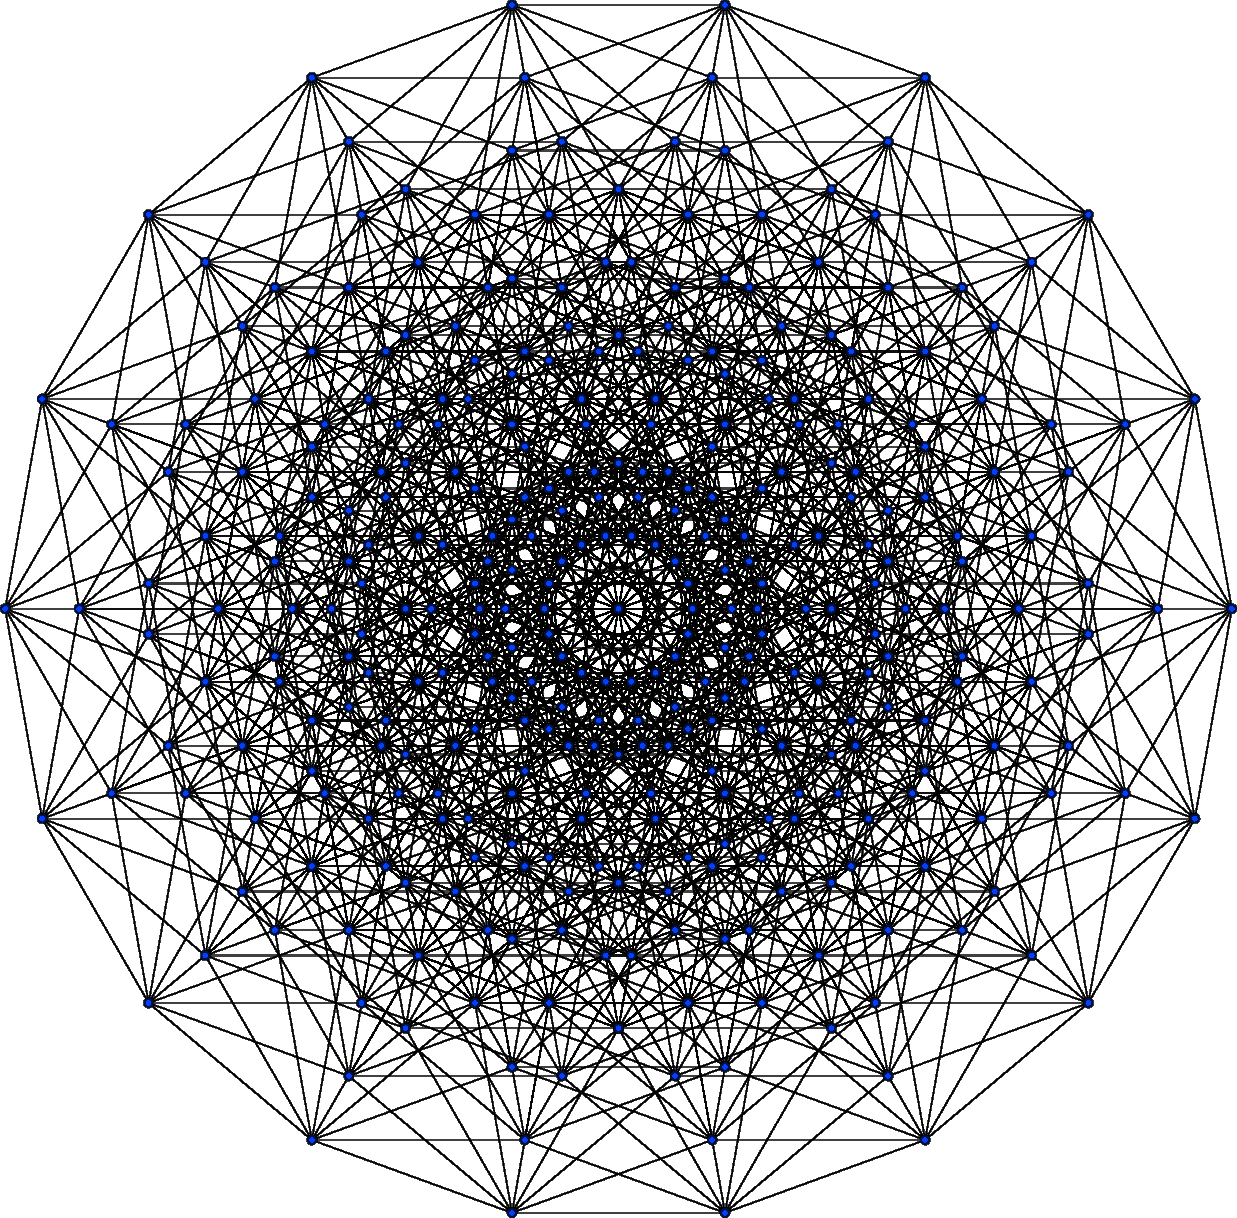
\includegraphics[scale=0.25]{images/q9.pdf}
\caption{Une projection de l'\textit{enneract} (9-cube)}
\end{figure}

\newpage

\subsection{Comparaison des différentes architectures}

À partir des résultats précédents, on peut manipuler les équations pour obtenir une estimation du diamètre, du degré des sommets, du nombre d'arêtes et de la bissection des différentes architectures étudiées jusqu'ici, directement en fonction du nombre de nœuds de calcul.

\begin{figure}[!h]
\begin{center}
\begin{tabular}{l|l|l|l|l}
Architecture & Diamètre & Degré & Nombre d'arêtes & Bissection \\ 
\toprule
Graphe complet & $1$ & $n-1$ & $\frac{n(n-1)}{2}$ & $\approx \frac{n^2}{4}$ \\ 
Grille de dimension $d$ & $d(n^{1/d}-1)$ & $2d$ & $dn(1-n^{-1/d})$ & $\approx n^{1-1/d}$ \\
Grille de dimension $2$ & $2(\sqrt{n}-1)$ & $4$ & $2(n-\sqrt{n})$ & $\approx \sqrt{n}$ \\ 
Grille d'arbres bidimensionnelle & • &  • & • & • \\ 
Hypercube & $\log_2 n$ & $\log_2 n$ & $\frac{1}{2}n\log_2 n$ & $\frac{n}{2}$ \\ 
\end{tabular}
\end{center}
\caption{Comparaison des architectures pour $n$ nœuds}
\end{figure}

On constate que l'hypercube offre les meilleurs diamètre et bissection, au détriment d'un degré non constant et d'arêtes plus nombreuses et plus longues par rapport à une grille classique, ce qui implique un câblage plus complexe et coûteux. Cela reste néanmoins une architecture de choix à l'heure actuelle.

\subsection{Template de communication}

On trouve dans \cite{FOSTER} un \textit{template} de communication classiquement utilisé dans de nombreux problèmes SIMD implémentés sur un hypercube :

\begin{algorithm}
\caption{hypercube($task\_id$, $n$, $input$, $output$)}
\begin{algorithmic}
\REQUIRE $task\_id$, $n$, $input$, $output$
\STATE $state \leftarrow input$
\FOR{$i = 0$ \TO $\log_2 n - 1$}
\STATE $partner \leftarrow task\_id \oplus 2^i$
\STATE $\text{send}(partner, state)$
\STATE $message \leftarrow \text{receive}(partner)$
\STATE $state \leftarrow \text{OP}(state, message)$
\ENDFOR
\STATE $output \leftarrow state$
\end{algorithmic}
\end{algorithm}

Cette procédure est exécutée par chacune des $n$ tâches. La tâche $task\_id$, dont l'état initial vaut $input$, communique avec ses $\log_2 n$ voisins qu'elle identifie simplement avec une opération XOR sur chaque dimension. Elle envoie son état courant à son partenaire et reçoit de ce dernier le sien. La tâche met à jour son état en effectuant une opération « OP » combinant son état courant et l'information reçue de son voisin.

\subsection{Tri bitonique}

Dans ce paragraphe, nous décrivons l'algorithme de tri par fusion bitonique, particulièrement adapté aux réseaux de tri et au calcul parallèle. Pour simplifier les explications, on considère un tableau de taille multiple de $n$, notée $l = Mn = M2^d$ avec $M$ entier. On commence par distribuer le tableau sur les $n$ nœuds d'un hypercube de dimension $d$, chaque nœud ayant pour état initial un sous-tableau de taille $M$.

Prenons par exemple le tableau de 24 éléments suivant : $[15, 10, 2, 11, 6, 4, 0, 3, 2, 13, 14, 7, 9, 9, 4, 13, 6, 5, 13, 0, 5, 2, 13, 1]$. On distribue ce tableau en 8 sous-tableaux de trois éléments, de manière arbitraire sur un hypercube de dimension 3 (figure \ref{fig:bitonic1}) puis chaque tâche trie ensuite, de manière séquentielle, son sous-tableau (figure \ref{fig:bitonic2}).

\begin{figure}[!h]
\begin{center}
\hspace*{-0.3in}
\begin{subfigure}[b]{0.45\textwidth}
\begin{tikzpicture}
\SetGraphUnit{3}
\GraphInit[vstyle=Normal]
\SetUpVertex[FillColor=blue!20]
\Vertex{000}
\EA(000){010}
\SO(000){001}
\EA(001){011}
\Vertex[x=1.5 , y=1.5]{100}
\EA(100){110}
\SO(100){101}
\EA(101){111}
\Edges(000,010,011,001,000)
\Edges(000,100,110,010)
\Edges(001,101,111,011)
\Edges(100,101)
\Edges(110,111)
\node[above left] at (-0.4, +0.2) {$[15,10,2]$};
\node[above left] at (-0.4, -3) {$[11,6,4]$};
\node[below right] at (+3.4, -3) {$[13,14,7]$};
\node[below right] at (+4.7, -1.8) {$[2,13,1]$};
\node[below right] at (+4.7, 1.2) {$[13,0,5]$};
\node[above left] at (+1.2, 1.8) {$[9,9,4]$};
\node[below right] at (+1.6, -1.8) {$[13,6,5]$};
\node[below right] at (+3.3, 0) {$[0,3,2]$};
\end{tikzpicture}
\caption{Distribution du tableau}
\label{fig:bitonic1}
\end{subfigure}%
\hfill
\begin{subfigure}[b]{0.45\textwidth}
\begin{tikzpicture}
\SetGraphUnit{3}
\GraphInit[vstyle=Normal]
\SetUpVertex[FillColor=blue!20]
\Vertex{000}
\EA(000){010}
\SO(000){001}
\EA(001){011}
\Vertex[x=1.5 , y=1.5]{100}
\EA(100){110}
\SO(100){101}
\EA(101){111}
\Edges(000,010,011,001,000)
\Edges(000,100,110,010)
\Edges(001,101,111,011)
\Edges(100,101)
\Edges(110,111)
\node[above left] at (-0.4, +0.2) {$[2,10,15]$};
\node[above left] at (-0.4, -3) {$[4,6,11]$};
\node[below right] at (+3.4, -3) {$[7,13,14]$};
\node[below right] at (+4.7, -1.8) {$[1,2,13]$};
\node[below right] at (+4.7, 1.2) {$[0,5,13]$};
\node[above left] at (+1.2, 1.8) {$[4,9,9]$};
\node[below right] at (+1.6, -1.8) {$[5,6,13]$};
\node[below right] at (+3.3, 0) {$[0,2,3]$};
\end{tikzpicture}
\caption{Tri séquentiel des sous-tableaux}
\label{fig:bitonic2}
\end{subfigure}
\end{center}
\caption{Initialisation du tri bitonique sur un hypercube ($M = 3$)}
\end{figure}

\subsubsection{\textit{Compare-split}}

Nous aurons besoin de faire communiquer les nœuds pour fusionner les sous-tableaux de manière à pouvoir obtenir la séquence triée attendue. L'idée est de maintenir des relations d'ordre sur les états des nœuds : pour des sous-tableaux $T_i$ et $T_j$ vivant respectivement sur les tâches $P_i$ et $P_j$, on écrira $T_i \leq T_j$ si chaque élément de $T_i$ est inférieur ou égal à chacun des éléments de $T_j$. On cherchera alors, pour deux nœuds voisins $P_i$ et $P_j$, à obtenir des sous-tableaux $T_i' \leq T_j'$ en combinant leurs sous-tableaux initiaux $T_i$ et $T_j$. L'algorithme permettant de réaliser cette opération porte le nom de \textit{compare-exchange} ou \textit{compare-split} et est notamment décrit dans \cite{GRAMA} :

\begin{enumerate}
\item Chaque tâche envoie à l'autre tâche son sous-tableau de $M$ éléments, si bien que les deux nœuds disposent d'une copie locale de $T_i$ et $T_j$.
\item Par un critère bien défini, chacune des tâches sait si elle joue le rôle de $P_i$ (resp. $P_j$) et fusionnera les deux tableaux $T_i$ et $T_j$ de manière à sélectionner les $M$ plus petits (resp. plus grands) éléments de $T_i \cup T_j$ (\textit{compare-split-high} ou \textit{compare-exchange-low}).
\item À l'issue, les deux tâches contiendront l'un des sous-tableaux $T_i'$ et $T_j'$ avec $T_i' \leq T_j'$ (et bien entendu $T_i' \cup T_j' = T_i \cup T_j$).
\end{enumerate}

\begin{figure}[!h]
\begin{center}\hspace*{-0.3in}
\begin{subfigure}[b]{0.30\columnwidth}
\begin{center}
\begin{tikzpicture}
\SetGraphUnit{4}
\GraphInit[vstyle=Normal]
\SetVertexMath
\SetUpVertex[FillColor=blue!20]
\Vertex{P_i}
\EA(P_i){P_j}
\Edge(P_i)(P_j)
\tikzstyle{VertexStyle} = [shape = rectangle,
                           draw = black,
                           fill = orange,
                           opacity = .35,
                           text opacity = 1,
                           inner sep = 2pt,
                           outer sep = 0.5pt,
                           minimum size = 6mm,
                           line width = 1pt]

\Vertex[x=0,y=0.9,L={[3,4,6]}]{1};
\Vertex[x=4,y=0.9,L={[0,2,9]}]{2};
\Edge[style={->,bend left=10},label=send/rcv](1)(2);
\Edge[style={->,bend left=10},label=rcv/send](2)(1);
\end{tikzpicture}
\caption{Les deux tâches s'envoient leur tableau}
\label{fig:bitonic3}
\end{center}
\end{subfigure}%
\hfill
\begin{subfigure}[b]{0.40\columnwidth}
\begin{center}
\begin{tikzpicture}
\SetGraphUnit{3}
\GraphInit[vstyle=Normal]
\SetVertexMath
\SetUpVertex[FillColor=blue!20]
\Vertex{P_i}
\EA(P_i){P_j}
\Edge(P_i)(P_j)
\tikzstyle{VertexStyle} = [shape = rectangle,
                           draw = black,
                           fill = orange,
                           opacity = .35,
                           text opacity = 1,
                           inner sep = 2pt,
                           outer sep = 0.5pt,
                           minimum size = 6mm,
                           line width = 1pt]

\Vertex[x=0,y=0.9,L={[3,4,6]}]{1};
\Vertex[x=3,y=0.9,L={[0,2,9]}]{2};
\Vertex[x=3,y=1.7,L={[3,4,6]}]{3};
\Vertex[x=0,y=1.7,L={[0,2,9]}]{4};
\Edge[style={->,bend left=100}](1)(4);
\Edge[style={->,bend left=100}](4)(1);
\Edge[style={->,bend left=100}](2)(3);
\Edge[style={->,bend left=100}](3)(2);
\end{tikzpicture}
\caption{Chaque tâche dispose d'une copie locale des deux tableaux, qu'elle fusionne}
\label{fig:bitonic4}
\end{center}
\end{subfigure}%
\hfill
\begin{subfigure}[b]{0.2\columnwidth}
\begin{center}
\begin{tikzpicture}
\SetGraphUnit{3}
\GraphInit[vstyle=Normal]
\SetVertexMath
\SetUpVertex[FillColor=blue!20]
\Vertex{P_i}
\EA(P_i){P_j}
\Edge(P_i)(P_j)
\tikzstyle{VertexStyle} = [shape = rectangle,
                           draw = black,
                           fill = orange,
                           opacity = .35,
                           text opacity = 1,
                           inner sep = 2pt,
                           outer sep = 0.5pt,
                           minimum size = 6mm,
                           line width = 1pt]

\Vertex[x=0,y=0.9,L={[0,2,3]}]{1};
\Vertex[x=3,y=0.9,L={[4,6,9]}]{2};
\end{tikzpicture}
\caption{Résultat\\~}
\label{fig:bitonic5}
\end{center}
\end{subfigure}
\end{center}
\caption{\textit{Compare-split} entre deux tâches $P_i$ et $P_j$}
\end{figure}

Les sous-tableaux initiaux étant triés, l'opération de fusion ne présente pas de difficulté et sa complexité est en $\mathcal{O}(M)$. Pour cette même raison, il n'est pas toujours nécessaire de disposer des $M$ éléments de l'autre sous-tableau pour obtenir le nouveau sous-tableau et on pourrait imaginer que les tâches s'échangent à la volée les éléments nécessaires à la décision, à condition que les coûts engendrés par le surplus de messages ne soient pas supérieurs aux gains liés à la réduction du volume des échanges.

\subsubsection{\textit{Parallel merge}}

\subsection{Quelques autres exemples d'algorithmes}